%%
% This is an Overleaf template for presentations
% using the TUM Corporate Desing https://www.tum.de/cd
%
% For further details on how to use the template, take a look at our
% GitLab repository and browse through our test documents
% https://gitlab.lrz.de/latex4ei/tum-templates.
%
% The tumbeamer class is based on the beamer class.
% If you need further customization please consult the beamer class guide
% https://ctan.org/pkg/beamer.
% Additional class options are passed down to the base class.
%
% If you encounter any bugs or undesired behaviour, please raise an issue
% in our GitLab repository
% https://gitlab.lrz.de/latex4ei/tum-templates/issues
% and provide a description and minimal working example of your problem.
%%

\documentclass[
  german,            % define the document language (english, german)
  aspectratio=169,    % define the aspect ratio (169, 43)
  % handout=2on1,       % create handout with multiple slides (2on1, 4on1)
  % partpage=false,     % insert page at beginning of parts (true, false)
  % sectionpage=true,   % insert page at beginning of sections (true, false)
]{tumbeamer}


% load additional packages
\usepackage{booktabs}
\usepackage{graphicx}
\usepackage{tikz}
\usepackage{url}
\usepackage{pgfplots}
\usepackage{hyperref}
\usepackage{pmboxdraw}
\usepackage{float}
\usepackage{babel}[ngerman]
\usepackage{csquotes}[autostyle]
\usepackage[useregional]{datetime2}
\usepackage{listings}
\input{../template/riscv}

\lstset {
    frame=single,
    tabsize=4,
    breaklines=true,
    xleftmargin=5pt,
    xrightmargin=5pt,
    basicstyle=\ttfamily\footnotesize,
    %language=[RISC-V]Assembler,
}


\hypersetup { 
  colorlinks=true,
  urlcolor=blue,
  filecolor=black,
  linkcolor=black
}

% tikz  
\usetikzlibrary{fit}

% image path
\graphicspath{ {../resources/} }

% presentation metadata
\title{Übung 03: RISC-V Deep Dive}
\subtitle{Einführung in die Rechnerarchitektur}
\author{\theAuthorName}

\institute{\theGroupName\\\theSchoolName\\\theUniversityName}
\date{04. -- \DTMdisplaydate{2024}{11}{10}{-1}}

\footline{\insertauthor~|~\insertshorttitle~|~\insertshortdate}


% macro to configure the style of the presentation
\TUMbeamersetup{
  title page = TUM tower,         % style of the title page
  part page = TUM toc,            % style of part pages
  section page = TUM toc,         % style of section pages
  content page = TUM more space,  % style of normal content pages
  tower scale = 1.0,              % scaling factor of TUM tower (if used)
  headline = TUM threeliner,      % which variation of headline to use
  footline = TUM default,         % which variation of footline to use
  % configure on which pages headlines and footlines should be printed
  headline on = {title page},
  footline on = {every page, title page=false},
}


% available frame styles for title page, part page, and section page:
% TUM default, TUM tower, TUM centered,
% TUM blue default, TUM blue tower, TUM blue centered,
% TUM shaded default, TUM shaded tower, TUM shaded centered,
% TUM flags
%
% additional frame styles for part page and section page:
% TUM toc
%
% available frame styles for content pages:
% TUM default, TUM more space
%
% available headline options:
% TUM empty, TUM oneliner, TUM twoliner, TUM threeliner, TUM logothreeliner
%
% available footline options:
% TUM empty, TUM default, TUM infoline


\begin{document}

\maketitle

\begin{frame}[c]{Mitschriften \& Infos}{}
  \begin{minipage}[t]{\textwidth}
    \begin{columns}[c]
      \begin{column}{0.8\textwidth}
        Montags: \href{\zulipMo}{\zulipMo}
      \end{column}
      \begin{column}{0.2\textwidth}
        \includegraphics[width=0.8\linewidth]{\zulipMoQrFilename}
      \end{column}
    \end{columns}
  \end{minipage}
  \rule{\textwidth}{0.4pt}
  \begin{minipage}[t]{\textwidth}
    \begin{columns}[c]
      \begin{column}{0.8\textwidth}
        Donnerstags: \href{\zulipDo}{\zulipDo}
      \end{column}
      \begin{column}{0.2\textwidth}
        \includegraphics[width=0.8\linewidth]{\zulipDoQrFilename}
      \end{column}
    \end{columns}
  \end{minipage}
  \ifdefined\myWebsite
  \rule{\textwidth}{0.4pt}
  \centering
  Website: \href{\myWebsite}{\myWebsite}
  \fi
\end{frame}

\begin{frame}[c]{}{}
  \begin{center}
    \LARGE  Keine Garantie für die Richtigkeit der Tutorfolien.

    \Large Bei Unklarheiten/Unstimmigkeiten haben VL/ZÜ-Folien recht!
  \end{center}
\end{frame}

\begin{frame}[fragile]{Hausaufgabe 02: mul\_pi\_16\_16}
  \framesubtitle{Code}
  \begin{lstlisting}
  li a1, 0x3243F              # pi in 16.16 (pi*65536)
  
  mulh t1, a0, a1             # high 32 bit of pi*x
  mul t0, a0, a1              # low 32 bit of pi*x
  
  srli t0, t0, 16             # shift low bits to the right
  slli t1, t1, 16             # shift high bits to the left
  or a0, t0, t1               # or the shifted registers
  
  jalr zero, 0(ra)            # return
  \end{lstlisting}
\end{frame}
  

\begin{frame}[c]{Inhaltsübersicht}{}
  \begin{columns}[c]
    \begin{column}{1\textwidth}
      \begin{itemize}
        \item Quiz
        \item Kurze Wiederholung
        \item Tutorblatt
        \begin{itemize}
          \item Arrays und deren Adressierung
          \item Strings
          \item Taschenrechner-Tester (Präsenzaufgabe 01)
        \end{itemize}
      \end{itemize}
    \end{column}
  \end{columns}
\end{frame}

\begin{frame}[c]{Abstraktionsebenen}{}
  \begin{columns}[c]
    \begin{column}{0.6\textwidth}
      \begin{itemize}
        \item Code in einer Hochsprache (C, Java, \textellipsis) ist lediglich eine Abstraktion
        \item Compiler: Hochsprache $\rightarrow$ Assemblersprache
        \item Assembler: Assemblercode $\rightarrow$ Maschinensprache (1:1 Übersetzung)
        \item Maschinensprache ist plattformspezifisch!
        \item ISA: \enquote{Bedienungsanleitung} einer CPU
        \item RISC vs. CISC
      \end{itemize}
    \end{column}
    \begin{column}{0.3\textwidth}
      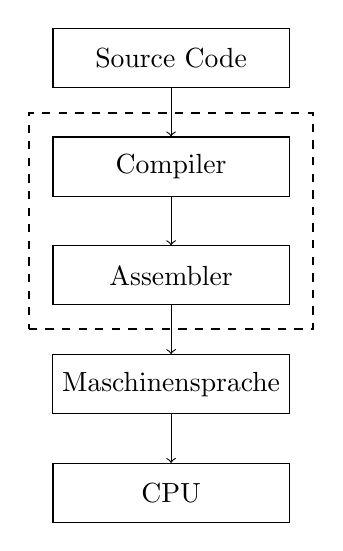
\begin{tikzpicture}[
          block/.style = {draw, rectangle, minimum width=3cm, minimum height=0.75cm, align=center},
          node distance=1.2cm
        ]

        \node[block] (source) at (0,0) {Source Code};
        \node[block, yshift=-1cm] (compiler)  at (source.south){Compiler};
        \node[block, yshift=-1cm] (assembler) at (compiler.south){Assembler};
        \node[block, yshift=-1cm] (machine) at (assembler.south) {Maschinensprache};
        \node[block, yshift=-1cm] (cpu) at (machine.south) {CPU};

        \draw[->] (source) -- (compiler) node[midway, right] {};
        \draw[->] (compiler) -- (assembler) node[midway, right] {};
        \draw[->] (assembler) -- (machine) node[midway, right] {};
        \draw[->] (machine) -- (cpu) node[midway, right] {};

        \node[draw, dashed, thick, inner sep=0.3cm, fit=(compiler) (assembler)] {};
      \end{tikzpicture}
    \end{column}
  \end{columns}
\end{frame}

\begin{frame}[c]{RISC-V}{}
  \begin{columns}[c]
    \begin{column}{0.5\textwidth}
      \begin{itemize}
        \item eine von vielen Assemblersprachen
        \item Datenwortbreite: 32 Bit (4 Byte)
        \item Little-Endian-Architektur
        \item 32 Register, einige davon mit spezieller Funktion
        \item grundlegende Instruktionen auf 32 Bit begrenzt 
        $\rightarrow$ Konstanten müssen zusammengebastelt werden
      \end{itemize}
    \end{column}
    \begin{column}{0.5\textwidth}
      \includegraphics[width=\linewidth]{riscv_registers.png}
    \end{column}
  \end{columns}
\end{frame}

\begin{frame}[c]{Addition}{}
  \begin{minipage}[t]{\textwidth}
    % Obere Hälfte für den Text
    \vspace{0.2cm} % optionaler Abstand zum Seitenrand
    \begin{itemize}
      \item addi kann zum Laden von Konstanten verwendet werden
      \item "Nur"\/  12-Bit Immediate
      \item Sign extension
    \end{itemize}
  \end{minipage}

  \vfill % Flexibler Abstand zwischen den Hälften

  \begin{minipage}[b]{\textwidth}
    % Untere Hälfte für das Bild
    \centering
    \includegraphics[width=1\linewidth]{add_sub.png}
  \end{minipage}
\end{frame}

\begin{frame}[c]{Laden von großen Konstanten}{}
  \begin{columns}[c]
    \begin{column}{1\textwidth}
      \begin{itemize}
        \item lui, rd, upimm
        \begin{itemize}
          \item upimm hat 20 Bit
          \item upimm wird zuerst um 12 nach links geshifted
          \item dann die unteren 12 Bit mit Null überschrieben
          \item anschließend Ergebnis nach rd geschrieben
        \end{itemize}
        \item Zum Laden von großen Konstanten zuerst lui, dann addi
        \item Achtung: Sign-Extension von addi kann zu unerwarteten Ergebnissen führen
        \item Pseudobefehl: li
      \end{itemize}
    \end{column}
  \end{columns}
\end{frame}

\begin{frame}[c]{Sign extension}{}
  \begin{minipage}[t]{\textwidth}
    % Obere Hälfte für den Text
    \vspace{0.2cm} % optionaler Abstand zum Seitenrand
    \begin{itemize}
      \item 12-Bit Konstante wird auf 32-Bit vergrößert, da Hardware nur mit 32-Bit Zahlen rechnet
      \item Die spezifizierten 12-Bit werden kopiert und die restlichen Stellen mit dem MSB (Sign Bit) aufgefüllt
      \item $\rightarrow$ Auffüllen mit 0, wenn Zahl positiv
      \item $\rightarrow$ Auffüllen mit 1, wenn Zahl negativ
    \end{itemize}
  \end{minipage}

  \vfill % Flexibler Abstand zwischen den Hälften

  \begin{minipage}[b]{\textwidth}
    % Untere Hälfte für das Bild
    \centering
    \includegraphics[width=0.75\linewidth]{signextension.png}
  \end{minipage}
\end{frame}

\begin{frame}[c]{Linksshift}{}
  \centering
  \includegraphics[width=0.75\linewidth]{unsiged_leftshift.png}
\end{frame}

\begin{frame}[c]{Rechtsshift}{}
  \centering
  \includegraphics[width=0.75\linewidth]{unsigned_rightshift.png}
\end{frame}

\begin{frame}[c]{}{}
  \begin{center}
    \LARGE Fragen?
  \end{center}
  \vspace{0.5cm}
  \begin{center}
    \LARGE Bis zum nächsten Mal ;) \\
  \end{center}
  \vspace{1.0cm}
  \begin{center}
    \small Folien inspiriert von Niklas Ladurner
  \end{center}
\end{frame}

\end{document}